\section{Оцінювання}
\label{sec:evaluation}

Оцінювання розділяє обчислювальну відтворюваність, поведінку детермінованих контрактів, описові вимірювання корпусу та семантичну правильність. Ці категорії мають різні еталони. Побайтово ідентичне повторне виконання встановлює повторюваність перетворення; негативний контроль --- відхилення заданого недійсного входу; жодне з них не встановлює істинності реконструйованої події. У таблиці~\ref{tab:evaluation} наведено всі десять системних експериментів із категорією доказів і межами, що лишаються. Машинозчитувані значення, хеші джерел, знаменники, середовище й команди супроводжують статтю у файлі \texttt{audited\_evaluation\_metrics.json}; журнали виконання зберігаються окремо. Для цих перевірок не знадобилося свіжого збору чи виконання моделей.

\begin{table}[!htbp]
\centering
\small
\caption{Матриця оцінювання системи. «Оцінено» означає вказане обмежене вимірювання, а не незалежну семантичну валідацію. Історичні квитанції відрізняються від свіжих перевірок.}
\label{tab:evaluation}
\begin{tabularx}{\textwidth}{@{}p{0.07\textwidth}p{0.19\textwidth}XX@{}}
\toprule
ID & Експеримент & Докази й спостережений результат & Межа оцінювання \\
\midrule
E1 & Відтворюваність & Свіжі перевірки хешів, повторне обчислення точного графа, арифметика збережених вибірок і чотири префікси по 25 вибірок збігаються. & Без свіжого повторного збору; повна генерація 9\,999 вибірок --- історична квитанція. \\
E2 & Збір даних & Збережені історичні й розширені підрахунки та пропуски незалежно перераховано. & Опис цілісності й охоплення; повнота платформ і повнота релевантності невідомі. \\
E3 & Виявлення дублікатів & Точний прохід: 369 пар, що відповідають умові; застарілі кандидати зберегли 367; два пропуски, нуль зайвих. & Умовна повнота кандидатів на скінченному корпусі; семантичного еталона дублікатів немає. \\
E4 & Виявлення координації & Збережена сім'я з 16 тестів: сире $p=0{,}0001$, $p$ за Голмом $=0{,}0016$; обмежені префікси відтворюються. & Умовні розвідувальні нульові моделі; специфічність щодо органічних подій і атрибуція не виміряні. \\
E5 & Пошук доказів & Пошук по зібраному корпусу та контролі посилань перевірено офлайн-тестами. & Кураторські відомі входи; сліпого бенчмарка пошуку у відкритому вебі немає. \\
E6 & Перевірка тверджень & Контрактні контролі утримання від рішення, конфлікту, граничного часу й ліній походження пройдено. & Незалежної оцінки семантичної точності чи випливання немає; авторський стрес-тест пізнішої ревізії правила наведено в розділі~\ref{sec:rule-v2}. \\
E7 & Реконструкція подій & Перевірено типізоване впорядкування подій і синтетичні інваріанти часової шкали та посилань. & Без автономного виявлення подій із сирих даних і незалежно встановленої оцінки хронології. \\
E8 & Відео/ASR & Історична арифметика відносно наданого еталона: 185 помилок на 415 слів, micro-WER 44,58\%. & Обрані кліпи; незалежне походження еталонного прослуховування не встановлено. \\
E9 & Наскрізний процес & Два чисті повтори лише з пошуком лишаються частковими й неперевіреними; негативний контроль із висячою подією не проходить. & Два кандидати, без прийнятої підтримки, без згенерованого звіту; це не сліпе оцінювання інциденту. \\
E10 & Час і ресурси & Свіжий офлайн-набір: 7,84\,с, максимум RSS 328\,320\,КіБ; виміряно й обмежений аналітичний аудит. & Часткові локальні навантаження; без поточного бенчмарка GPU, вартості API чи пропускної здатності повного запуску. \\
\bottomrule
\end{tabularx}
\end{table}

Свіжий повний набір тестів репозиторію на зафіксованій базовій ревізії дав 783 пройдені тести й 16 пройдених підтестів без збоїв на робочій станції, яка зберігає приватні корпуси. Pytest зафіксував 7,41\,с; зовнішнє вимірювання ресурсів --- 7,84\,с реального часу й максимум резидентної пам'яті 328\,320\,КіБ з успішним завершенням. Інтерпретатором був Python 3.13.14 віртуального середовища репозиторію на Linux/x86-64. Ці підрахунки описують регресійне покриття, а не знаменник точності. Також пройдено шість зафіксованих синтетичних контролів: відомий мікрокейс, розгалуження копій із одного кореня, суперечливі свідчення, граничні часи виправлень, неповні докази й повторно використане відео. Їхні очікувані стани відомі за побудовою. Вони корисні як бар'єри випуску, але не є сліпими спостереженнями істинності інцидентів.

Для обліку збору пряме читання файлів звірило 23\,350 історичних публікацій із 1\,408 обраними релевантними записами та 1\,384 текстами, придатними для аналізу схожості. Історичні 459 відсутніх сирих текстів і 49 відсутніх лічильників переглядів належать до всіх публікацій; у релевантній підмножині жоден із цих показників не відсутній. Решта 24 релевантні тексти коротші за поріг придатності у 80 символів. Розширений знімок містить 23\,386 публікацій і 1\,438 релевантних записів. Ці версії є окремими рамками аналізу. Точний граф і умовні часові тести використовують історичну рамку; приписування цього графа розширеній рамці в документі ліній походження відхилено за його зафіксованими вхідними хешами. Такі перевірки стосуються цілісності знаменників, не встановлюючи репрезентативності вибірки~\cite{Olteanu2019,VicentePaula2023}.

Експеримент із дублікатами заново обчислив весь придатний точний граф за визначенням п'ятисимвольних шинглів із робочого коду та 64-бітною арифметикою перетинів. За порогів Jaccard 0,60, 0,75 і 0,90 точні міжканальні підсумки становили 369, 288 і 213; застарілий пошук зберіг 367, 288 і 213. Отже, повнота кандидатів за порогу 0,60 дорівнює $367/369=99{,}45799458\%$ за умови 1\,384 придатних історичних текстів. Вісімнадцять пар у межах одного каналу виключено визначенням графа. Обидва пропущені міжканальні ребра мають лаг понад 30 хвилин, тому спостережені короткі лаги лишаються 134 у межах десяти хвилин і 198 у межах тридцяти, кожен із них тепер поділено на 369. На рисунку~\ref{fig:copy} показано це розрізнення між пошуком кандидатів і точним вимірюванням. Скетчинг шинглів забезпечує механізм пошуку, а не семантичну тотожність чи залежність джерел~\cite{Broder1997}.

\begin{figure}[!htbp]
\centering
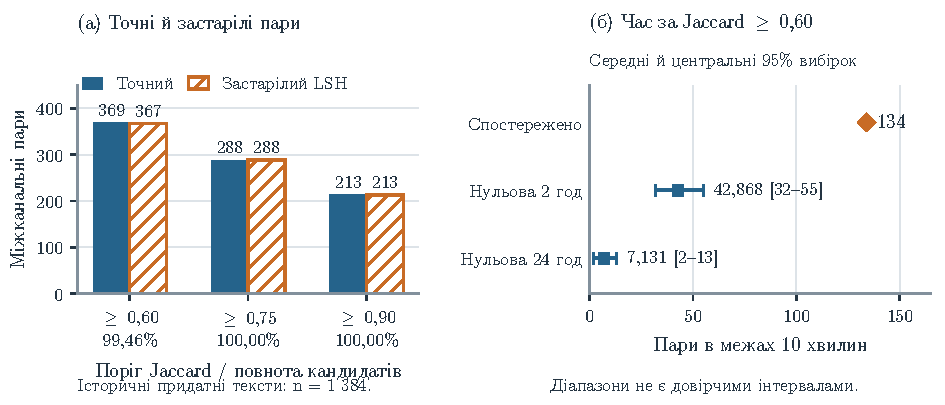
\includegraphics[width=\textwidth]{information_analysis.pdf}
\caption{Пошук схожості на скінченному корпусі та умовний час копіювання. Ліворуч: точні й збережені застарілим методом пари з повнотою для кожного порога серед 1\,384 придатних історичних текстів. Праворуч: 134 спостережені пари з Jaccard $\geq 0{,}60$ у межах десяти хвилин порівняно із середніми двох збережених умовних нульових моделей. Вуса показують центральні 95\% із 9\,999 рандомізованих вибірок, а не довірчі інтервали. Усі часові підрахунки використовують фіксований граф із 369 ребер. Джерела й хеші збережено в \texttt{data/figure\_data/information\_analysis.json}.}
\label{fig:copy}
\end{figure}

Для координації кожну збережену вибірку перечитано, а всі шістнадцять підсумкових рядків обчислено заново, зокрема середні, квантилі, верхні включні хвости й поправку на множинність. За 9\,999 вибірок усі зафіксовані кількості перевищень дорівнюють нулю; значення Монте-Карло з додаванням одиниці становить $(0+1)/(9999+1)=0{,}0001$, а поправка Голма для оголошеної сім'ї дає 0,0016~\cite{Phipson2010,Holm1979}. Свіже повторне виконання відтворило перші 25 вибірок кожної з чотирьох моделей із зерном 20261106. Цей аудит не генерував заново всі вибірки. Часові перестановки призначають кожному вузлу графа один зсунутий час, спільний для його ребер. Отже, ребра не трактуються як незалежні випробування. Відхилення від цих умовних фонів не встановлюють намір, неавтентичність, організатора чи специфічність щодо підібраних доброякісних подій~\cite{Pacheco2021,Nizzoli2021,Magelinski2022}.

Семантичне оцінювання лишається обмеженішим. Порівняння наративів зіставляє правила з мітками Claude на сорока обраних тестових дописах, а не з незалежним людським рішенням; його статистики узгодженості не можуть валідувати точність визначення позиції. Пошук доказів працює по зібраному корпусу, а лексичне ранжування не встановлює випливання уривка~\cite{RobertsonZaragoza2009BM25}. Кураторські регресійні перевірки тверджень і синтетичні контрприклади подано саме як такі. Типізовані записи подій упорядковують надані твердження; структурна дійсність не демонструє виявлення реальних фізичних подій. Так само історичний розрахунок помилки ASR використовує надані еталонні рядки, незалежне походження прослуховування яких не встановлено. Його micro-WER 44,58\% є описовою арифметикою для цих кліпів, а не сліпим бенчмарком розпізнавача на всьому корпусі.

Свіжий артефакт димової перевірки процесу фіксує два повторні запуски лише з пошуком: два кандидати, неперевірене твердження, нуль прийнятих оцінок підтримки й жодного звіту. Третій запуск навмисно вводить висяче посилання на докази події та коректно не проходить оцінювальний бар'єр. Однакові семантичні проєкції у чистих повторах встановлюють обмежену повторюваність, а їхній частковий статус вказує на незавершені етапи. Поєднаний аналітичний аудит тривав 4,8317\,с із максимумом RSS 1\,032\,620\,КіБ, включно із завантаженням корпусу, точним порівнянням, перевіркою збережених вибірок, відтворенням префіксів і реконструкцією графа й інтервалів. Ці вимірювання ресурсів не охоплюють збір, робочий ASR, зовнішні моделі та подальші допоміжні перевірки. Поточний час GPU чи грошову вартість API не вимірювали. Незалежна точність доказів, подій і звітів на рівні інцидентів тому лишається невиміряним результатом, а не виведеною перевагою успішного набору тестів.

\subsection{Післяаудитна ревізія правила відношень}\label{sec:rule-v2}
Наведені вище результати описують зафіксовану базову ревізію. Оскільки контрприклади зачіпають єдиний шлях, що створює прийняті оцінки доказів, одну оприлюднену зміну зроблено після аудиту й оцінено окремо. Ревізія \code{319d205} (ідентифікатор правила \code{rule_autonomous_claim_matcher_v2}) не надає підтримки, якщо не виконано три умови: кожне заявлене значення трапляється в одному реченні уривка, яке також має щонайменше дві спільні із твердженням змістові словоформи; уривок не заперечує змістове слово, яке стверджує твердження; і прізвище будь-якої пари суміжних імен із великої літери у твердженні наявне в уривку. Утримані пари лишаються неприйнятими кандидатами й не перетворюються на суперечності. Загальний офлайн-запускач не змінено, і він досі нічого не приймає автоматично.

\begin{table}[!htbp]
\caption{Детермінований стрес-тест правила відношень на випадках, виведених із 25 кураторських тверджень. Клітинки рахують пари, прийняті як підтримка. Очікувані результати виконуються за побудовою, крім зазначених у тексті; це не сліпий бенчмарк точності.}\label{tab:rule-v2}
\centering\small
\begin{tabularx}{\textwidth}{@{}YrrrY@{}}
\toprule
Сім'я випадків & $n$ & База & Ревізія & Очікуваний результат\\
\midrule
Незмінені прийняті пари (контроль) & 22 & 22 & 19 & Збереження, а не правильність\\
Хибний присудок, те саме число & 27 & 27 & 0 & Немає підтримки\\
Заперечений присудок & 9 & 9 & 0 & Немає підтримки\\
Змінене число & 7 & 0 & 0 & Немає підтримки\\
Уривок з іншого твердження & 469 & 5 & 2 & Немає підтримки; див. текст\\
\bottomrule
\end{tabularx}
\end{table}

У таблиці~\ref{tab:rule-v2} порівняно обидві версії правила на 534 детермінованих випадках, згенерованих \code{evaluate_verifier_challenges.py}. Базова версія прийняла всі 27 випадків із хибним присудком і всі дев'ять заперечених; ревізія не прийняла жодного. Читання двох прийнятих міжтвердженнєвих випадків, що лишилися, показує: обидва уривки містять заявлений зміст (четверо військових ідуть до швидкої та тримання під вартою названої підозрюваної), тож це дефекти побудованої негативної мітки, а не хибна підтримка. Із 22 контрольних пар прийнятими лишаються 19. Дві з трьох відкликаних пар --- уривки про травми й пересування, процитовані для твердження про самовільне залишення частини. Третя є ціною запобіжника щодо імен: уривок про заставу правильно вказує суму, але не називає особу.

Повторний запуск пакета записує новий артефакт і лишає файл від 9 листопада незмінним. Переглянутий результат містить 18 підтриманих, сім із недостатніми доказами й нуль спростованих результатів із 33 прийнятих оцінок; твердження про судову заставу --- єдина зміна статусу. Після цього набір тестів репозиторію проходить 794 тести й 16 підтестів. Одне ШІ-прочитання 19 пар підтримки, що лишилися, не виявило явної хибної підтримки, але виявило дві слабкі пари: одна прирівнює «два місяці» до 60 днів через закодоване правило, друга повідомляє, що персонал швидкої викликав поліцію, а не що поліція прибула. Таке прочитання не є незалежним рішенням.

Ці результати показують, що два задокументовані класи збоїв закрито на перевірених формах. Вони не оцінюють помилку на реальному тексті. Випадки написано після того, як збої стали відомими, тією самою ШІ-системою, яка переглянула правило, на основі трьох шаблонів і одного генератора заперечень. Перефразування, неявне заперечення, застережні формулювання й присудки, що охоплюють кілька речень, не перевірялися, а фіксована впевненість 0,92 лишається некаліброваною.
